\documentclass[11pt]{article}
\usepackage{amsmath,amssymb,mathtools}
\usepackage{bm}
\usepackage{siunitx}
\usepackage{geometry}
\usepackage{pgfplots}
\pgfplotsset{compat=1.18}
\geometry{margin=1in}
\title{Spectral Analysis with Windowing and FFT: Mathematical and Physical Intuition}
\author{}
\date{}

\begin{document}
\maketitle

\section*{Introduction}
The purpose of short-time Fourier analysis is to extract the frequency content of a time-varying signal
such as sound. Although Fourier theory provides a clean decomposition of infinite, perfectly periodic
signals, real-world audio is finite, sampled, and only available in short blocks. This creates
\emph{spectral leakage}, which motivates the use of window functions such as the Hann window. This
document provides both mathematical formulas and physical intuition.

\section*{Spectral leakage}
Suppose we measure a sinusoid
\begin{equation}
    x(t)=\cos(2\pi f_0 t)
\end{equation}
for a finite time $T$. Multiplying by a rectangular window
\begin{equation}
    w_T(t)=
    \begin{cases}
        1 & 0\le t<T,         \\
        0 & \text{otherwise},
    \end{cases}
\end{equation}
corresponds in the frequency domain to a convolution of a perfect Dirac peak at $f_0$ with the
Fourier transform of $w_T(t)$, which is a sinc function. Physically, this means the energy of a
single sinusoid ``spills'' into many nearby frequencies instead of appearing as one infinitely sharp
line. This phenomenon is called \emph{spectral leakage}.

\begin{figure}[h]
    \centering
    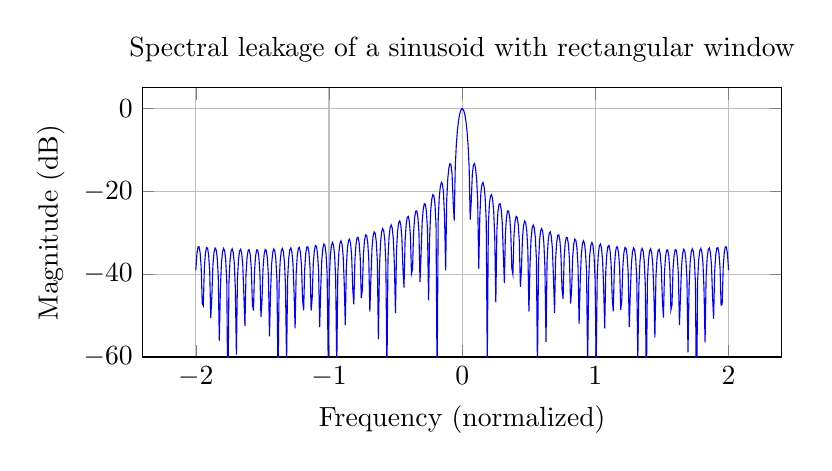
\begin{tikzpicture}
        \begin{axis}[
                width=0.8\textwidth,
                height=5cm,
                xlabel={Frequency (normalized)},
                ylabel={Magnitude (dB)},
                ymin=-60,ymax=5,
                grid=both,
                title={Spectral leakage of a sinusoid with rectangular window}
            ]
            \addplot+[mark=none,domain=-2:2,samples=500] {20*log10(abs(sin(deg(50*x))/(50*sin(deg(x)))))};
        \end{axis}
    \end{tikzpicture}
    \caption{Sinc-shaped spectrum of a finite sinusoid. Energy leaks into distant bins.}
\end{figure}

\section*{The Hann window: definition and purpose}
To reduce leakage, one applies a smooth apodization function before Fourier analysis. The Hann
(Hanning) window is defined by
\begin{equation}
    w[n]=\tfrac{1}{2}\left(1-\cos\frac{2\pi n}{N-1}\right),\qquad 0\le n<N,
\end{equation}
where $N$ is the frame length. This function smoothly ramps up from $0$ to $1$ and back to $0$,
avoiding the discontinuities of the rectangular cut-off. Its Fourier transform has significantly
lower sidelobe levels (about $-31$\,dB), so leakage into distant frequencies is suppressed.

\paragraph{Physical intuition.} Applying a Hann window is analogous to tapering the edges of a finite
measurement to avoid introducing sharp boundaries, much like how diffraction is reduced when an
aperture is smoothly apodized instead of sharply truncated.

\begin{figure}[h]
    \centering
    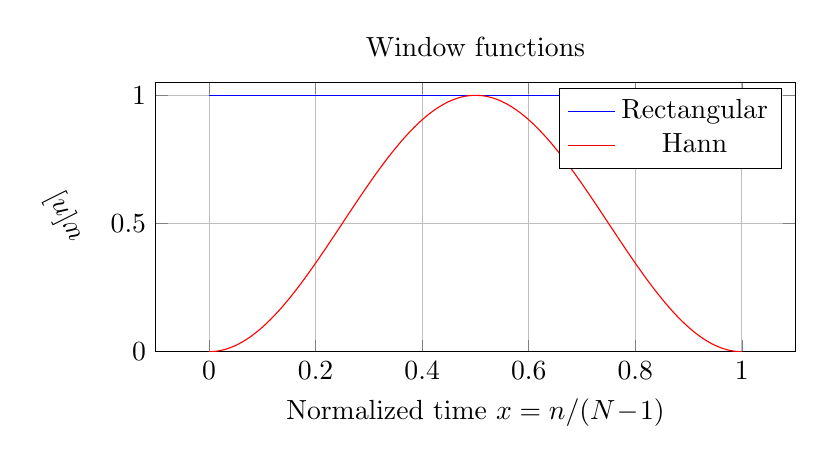
\begin{tikzpicture}
        \begin{axis}[
                width=0.8\textwidth,
                height=5cm,
                xlabel={Normalized time $x = n/(N\!-\!1)$},
                ylabel={$w[n]$},
                ymin=0, ymax=1.05,
                grid=both,
                title={Window functions},
                trig format=rad       % <-- key fix: interpret trig in radians
            ]
            \addplot+[mark=none,domain=0:1,samples=400] {1};                 % Rectangular window
            \addplot+[mark=none,domain=0:1,samples=400] {0.5*(1 - cos(2*pi*x))}; % Hann window
            \legend{Rectangular,Hann}
        \end{axis}
    \end{tikzpicture}
    \caption{Rectangular vs. Hann windows. The Hann window smoothly tapers edges (raised cosine).}
\end{figure}

\section*{Short-Time Fourier Transform}
Given a discrete-time signal $x[n]$, we analyze overlapping frames:
\begin{equation}
    \tilde{x}_m[n]=w[n]\,x[n+mH],\quad 0\le n<N,
\end{equation}
where $H$ is the hop size (step between frames). Each frame is Fourier transformed:
\begin{equation}
    X_m[k]=\sum_{n=0}^{N-1}\tilde{x}_m[n]\,e^{-j2\pi kn/N}.
\end{equation}
Here $k$ indexes frequency bins with physical frequency $f_k=k f_s/N$, where $f_s$ is the sampling
rate.

\paragraph{Physics interpretation.} The STFT provides the instantaneous frequency spectrum of the
signal, analogous to decomposing a time-dependent wave into its Fourier modes, but restricted to a
moving finite observation window. It balances time resolution ($H,f_s$) against frequency resolution
($N$).

\section*{Time--frequency trade-off}
Because the frame length $N$ fixes both duration $T=N/f_s$ and frequency resolution $\Delta f=f_s/N$,
there is a trade-off: longer windows give sharper frequency peaks but blur fast temporal changes,
and shorter windows give precise timing but poorer frequency discrimination.

\begin{figure}[h]
    \centering
    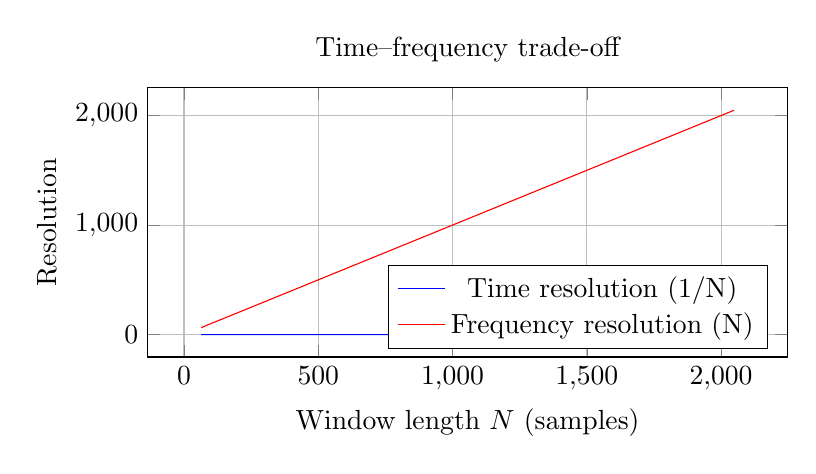
\begin{tikzpicture}
        \begin{axis}[
                width=0.8\textwidth,
                height=5cm,
                xlabel={Window length $N$ (samples)},
                ylabel={Resolution},
                legend pos=south east,
                grid=both,
                title={Time--frequency trade-off}
            ]
            \addplot+[mark=none,domain=64:2048,samples=100] {1/x}; % time resolution ~1/N
            \addplot+[mark=none,domain=64:2048,samples=100] {x};   % freq resolution ~N
            \legend{Time resolution (1/N),Frequency resolution (N)}
        \end{axis}
    \end{tikzpicture}
    \caption{Increasing window length improves frequency resolution but worsens time resolution.}
\end{figure}

\section*{Quadratic interpolation of peaks}
Because FFT bins are discrete, the true sinusoidal frequency $f_0$ may lie between bins. To estimate
this, we fit a parabola through the logarithmic magnitudes at $k-1,k,k+1$ and extract the vertex
offset $\Delta$:
\begin{equation}
    \Delta=\tfrac{1}{2}\frac{M[k-1]-M[k+1]}{M[k-1]-2M[k]+M[k+1]},\qquad \hat f=\frac{k+\Delta}{N}f_s.
\end{equation}
This procedure recovers a sub-bin estimate of frequency. Physically, it amounts to estimating the
location of the peak of a sinc lobe more accurately than the FFT grid allows.

\section*{Harmonic structure and timbre}
For quasi-periodic signals (e.g.\ musical tones, voiced speech), energy appears at integer multiples
of a fundamental frequency $f_0$. One may extract a \emph{timbre vector}
\begin{equation}
    \bm{t}=\big(M[k_1],M[k_2],\dots\big),
\end{equation}
where $k_h\approx h f_0 N/f_s$. This vector characterizes the relative strength of harmonics and
thus the perceptual color of the sound.

\section*{Summary}
\begin{itemize}
    \item Spectral leakage arises from the finite-time observation of signals, spreading energy into
          sidelobes.
    \item Window functions (Hann) smooth the edges, lowering sidelobe levels while widening the main lobe,
          trading frequency resolution for cleaner separation of tones.
    \item The STFT provides a time--frequency decomposition, balancing temporal and spectral resolution.
    \item Quadratic interpolation refines frequency estimates beyond FFT bin width.
    \item Harmonic vectors summarize timbre, linking physics of periodic excitation and system response
          to perceptual sound quality.
\end{itemize}

\end{document}